% Hoda Abbasi
% 16 March 2016

\documentclass[]{book}
\input Latex_macros/Definitionen.tex
\usepackage{a4}
\usepackage{graphicx}
\usepackage{tikz-qtree}
\usepackage[active]{srcltx}
\usepackage[all]{xy}
\usepackage{enumerate}

\setcounter{tocdepth}{4}
\setcounter{secnumdepth}{4}
\newcommand{\Schrift}{report}

\begin{document}
\title{Hardness measures of clause-sets}

\author{Hoda Abbasi\\
        PhD Candidate\\
        Computer Science Department\\
        Swansea University\\}
\maketitle

\tableofcontents
%%%%%%%%%%%%%%%%%%%%%%%%%%%%%%%%%%%%%%%%%%%%%%%%%%%%%%%%%%
\chapter{Introduction}
\label{cha:Introduction}

The aim of this report is to investigate different hardness measures for a clause-set in the literature and then, to propose a method based on Prover-Delayer games. 

The report is organized as follows. In Chapter \ref{cha:Preliminaries} some general preliminaries are presented. Then, in Chapter \ref{cha:Hardness Measures} hardness is defined as a measure for complexity of unsatisfiable clause-set. This measure, then is extended for arbitrary clause-set. Chapter \ref{cha:XOR-constraints} explains a system of XOR-constraint and ??????

In Chapter \ref{cha:hdgame}, the proposed method to obtain the hardness of a clause-set is given. Finally, Chapter \ref{cha:concl} presents some questions regarding hardness measures and the hardness game and then, it concludes the report.
%%%%%%%%%%%%%%%%%%%%%%%%%%%%%%%%%%%%%%%%%%%%%%%%%%%%%%%%%%
\chapter{Preliminaries}
\label{cha:Preliminaries}

\section{Clause-sets}
\label{sec:Clause-sets}

The infinite set of variables is denoted by $\Va$. A partial assignment $\vp$ is a map which assigns a unique value in $\{0,1\}$ to each elemet of a finite set of variables. The domain of this map is a set of variables denoted by $\var(\vp)$. The set of all partial assignments is indicated by $\Pass$ and for $V \in \pote(\Va)$, $\Tass(V)$ is the set of total assignments over $V$. The empty partial assignment is denoted by $\epa:= \es \in \Pass$. For a partial assignment $\vp \in \Pass$, the number of variables is defined as $n(\vp):=\abs{\var(\vp)}$. For two partial assignments $\vp, \psi \in \Pass$, the composition operation is defined as $\vp \circ \psi := \psi \cup (\vp \sm \var(\psi)) \in \Pass$ which is the union of their variables if they do not conflict. In the case of conflicting variables, the second assignment is considered. This operation has associative property and it is commutative if $\vp, \psi$ do not clash.

A literal is a pair $(v,\ve)$ with $\var((v,\ve)):=v \in \Va$ and $\val((v,\ve)):=\ve \in \{0,1\}$. The set of all literals is $\Lit$. Two literals $x, y \in \Lit$ clash if they have a same variable but different values. For a set $L \sse \Lit$ we define $\var(L) := \set{\var(x) : x \in L}$, $\lit(L):= \set{x \in \Lit : \var(x) \in \var(L)}$ and $\ol{L} := \lit(L) \sm L$. A clause is defined as a finite and clash-free set of literals. The set of all clauses is denoted by $\Cl$ and $\bot := \es \in \Cl$ is the empty clause. 

A clause-set is a finite set of clauses and $\Cls$ is the set of all clause-sets. The empty clause-set is indicated by $\top := \es \in \Cls$. For $F \in \Cls$ we define $\var(F) := \bc_{C \in F} \var(C) \in \pote(\Va)$ and $\lit(F) := \var(F) \cup \ol{\var(F)}$. The number of variables in $F$ is denoted by $n(F) := \abs{\var(F)} \in \NNZ$ and the number of clauses is $c(F) := \abs{F} \in \NNZ$. The number of literal occurrences in $F$ is also denoted by $\ell(F) := \sum_{C \in F} \abs{C} \in \NNZ$. If the union of literals occuring in $F$ is indicated by $\bigcup F \subset \Lit$, then a pure literal for $F \in \Cls$ is defined as $x \in \bigcup F$ and $\ol{x} \not \in \bigcup F$. A full clause $C$  for a clause-set $F$ is defined as $C \in F$ and $\var(C) = \var(F)$, and a clause-set $F$ is called full if every clause of $F$ is full. The full clause-set for a finite set of variables $V$ is denoted by $A(V)$. 

\begin{examp}\label{exp:An}
  If $A(V)$ for $V=\set{1,..., n}$ is indicated by $A_n$ then $A_0 = \set{\bot}$, $A_1 = \set{\set{1},\set{-1}}$ and $A_2 = \set{\set{-1,-2},\set{-1,2},\set{1,-2},\set{1,2}}$.
\end{examp}

Partial assignments are extended from variables to literals using $\vp(\ol{v})=\ol{\vp(v)}$. The operation of a partial assignment on a clause-set is defined as $\vp * F := \set{C \sm \vp : C \in F \wedge C \cap \ol{\vp} = \es} \in \Cls$. This means removing all clauses having at least one literal with $\vp (x)=1$ and then, removing from all clauses the literals with $\vp (x)=0$. A clause-set $F$ is called satisfiable if there exists a partial assignment $\vp$ such that $\vp * F = \top$. Another definition for a satisfiable clause-set $F$ is that there exists a clause which clashes with all clauses of $F$. The set of all satisfiable clause-sets is indicated by $\Sat := \set{F \in \Cls \mb \ex\, \vp \in \Pass : \vp * F = \top}$ while $\Usat := \Cls \sm \Sat$. If $\vp * F = \top$ then the partial assignment is called a satisfying assignment for $F$.

\section{Implication-relation}
\label{sec:imprel}

The implication-relation for two clause-sets $F, F'$ is defined as $F \models F'$ if $\fa\, \vp \in \Pass : \vp * F = \top \Ra \vp * F' = \top$. This relation can also be considered between a clause $C$ and a clause-set $F$ if $F \models \set{C}$ (which is indicated as $F \models C$). For  $F \in \Usat$ the only implication-relation is $F \models \bot$. 

A literal $x$ is called forced literal for a clause-set $F$ if $F \models x$ and $\pab{x \ra 1}$ is the forced assignment for $F$. A clause $C$ is called an implicate of a clause-set $F$ if $F \models C$ and it is called a prime implicate if there no $ C' \sse C$ as an implicate of $F$. The set of all prime implicates of $F$ is denoted by $\primec_0(F) \in \Cls$. A clause $C$ is called an implicant of a clause-set $F$ if $C$ as a partial assignment is a satisfying assignment for $F$. In other words, $C$ must fulfill $C * F=\top$. A prime implicant is a minimal implicant and the set of all prime implicants is indicated by $\primec_1(F) \in \Cls$. For example, for $F \in \Usat$ we have $\primec_0(F) = \set{\bot}$ and $\primec_1(F) = \top$.

\begin{examp}\label{exp:bbb}
For $F = \{\{ \neg x, y\} , \{ \neg y, z\}\}, prc_0(F) = \{\{\neg x, y\} , \{\neg y, z\} , \{\neg x, z\}\}$. Also for $F = \{\{x, y\} , \{x,\neg y\}\}, prc_0(F) = \{\{x\}\}$.
\end{examp}

Two clause-sets $F, G$ are called logically equivalent if $F \models G$ and $G \models F$. In this case, we have $\primec_0(F) = \primec_0(G)$ and $\primec_1(F) = \primec_1(G)$.

\section{Resolution}
\label{sec:Resolution}

The resolution is an operation applied to two clauses $C,D$ which clash in exactly one variable and produces a new clause. The result of the resolution for $C \cap \overline D = \{ x \}$ (which is called resolvent) is defined as $C \diamond D := (C \cup D) \setminus \{x, \overline x\} $. $C,D$ are called resolvable clauses and $x$ is the resolution literal.

Using the resolution operation, a resolution tree $T$ is produced for a clause-set $F$. The tree is indicated by $T : F \vdash C$ which clause $C$ is the root (conclusion) of $T$. The leaves of $T$ (axioms) are the clauses of $F$ and each inner node is the resolvent of its two parents. The number of nodes in $T$ is called tree-resolution complexity and denoted by $\comptr(R) \in \NN$. A resolution proof of a clause $C$ from a clause-set $F$ is a resolution tree $T : F \vdash C$. If a resolution refutation drives $\bot$, it is called a resolution proof and $F$ is unsatisfiable.

\begin{examp}\label{exp:res1}
A resolution tree for $F = \{\{a,b\},\{\neg a,b\},\{a, \neg b\},\{\neg a, \neg b\}\}$ is as Fig \ref{fig:resol1}. Since the empty clause is driven, it is called resolution refutation.
	   \begin{figure}
	   \centering  
       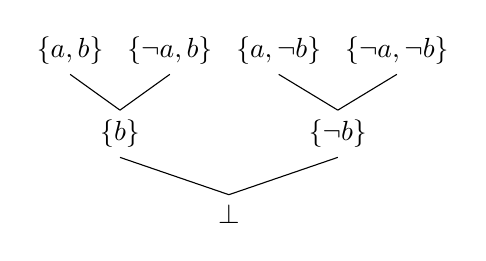
\begin{tikzpicture}[grow'=up]
       \Tree [.$\bot$  [.${\{b\}}$ ${\{a,b\}}$ ${\{\neg a,b\}}$ ] [.${\{ \neg b\}}$ ${\{a, \neg b\}}$ ${\{\neg a, \neg b\}}$ ] ]
       \end{tikzpicture}
	   \caption{A resolution tree for Example \ref{exp:res1}.}
	   \label{fig:resol1}
       \end{figure}
\end{examp}

\section{Generalised unit-clause propagation}
\label{sec:rkred}

A reduction is considered as a map $r: \Cls \ra \Cls$ such that for all $F \in \Cls$, $r(F)$ is satisfiability-equivalent to $F$. Using the reduction technique, unsatisfiability is resulted if $\bot \in r(F)$. An example of the reduction is unit resolution (or unit propagation) which is applied to a clause-set $F$ with at least one unit-clause (a clause with one literal). This technique is performed by setting the literal in unit-clause to its satisfying assignment. For example for clause $\set{x}$, we set the literal $x$ to true. If the reduction yields $\bot$, then $F$ is unsatisfiable. Else, if there are more unit-clauses, this step is continued untill no unit-clause is left.

Another case of the reduction is generalised unit-clause propagation introduced in \cite{h10} and denoted by $\rk_k$. This technique removes all forced literals using forced assignments and discovers unsatisfiability if $\bot \in \rk_k(F)$. If $\bot \not \in F$, for $k=1$ the generalised unit-clause propagation eliminates all unit-clauses with assigning their satisfying assignment. Thus, $\rk_1$ is the unit-clause propagation and all clauses in $\rk_1$ must have length at least $2$. The next level is to obtain $\rk_2$ which is called failed literal elimination since all unit-clauses have already been removed. In each level $k$, if $\rk_k$ yields $\bot$ the original clause-set $F$ is unsatisfiable while $F$ is satisfiable if $\top$ is obtained. In the latter case, the sequence of forced assignments eliminated untill that level is a satisfying assignment for $F$. This technique is not complete since if $\rk_k$ can discover the unsatisfiability of a clause-set $F$, then all clauses in $F$ must have size at least $K+1$.

\begin{defi}\label{def:rk}
\cite{h10} The maps $\rk_k: \Cls \ra \Cls$ for $k \in \NNZ$ are defined as follows (for $F \in \Cls$):
  \begin{eqnarray*}
  \rk_0(F) & := &
  \begin{cases}
  \set{\bot} & \text{if } \bot \in F\\ F & \text{otherwise}
  \end{cases}\\
  \rk_{k+1}(F) & := &
  \begin{cases}
  \rk_{k+1}(\pao x1 * F) & \text{if } \ex\, x \in \lit(F) : \rk_k(\pao x0 * F) = \set{\bot}\\ F & \text{otherwise}
  \end{cases}.
  \end{eqnarray*}
\end{defi}

\begin{examp}\label{exp:rk}
Using literals $a,b,c,d$, $\rk_k(F)$ for some examples is computated as follows:
  \begin{enumerate}
  \item $\rk_k(\set{\bot}) = \set{\bot}$ for $k \ge 0$ and $\rk_k(\top) = \top$ for $k \ge 0$.
  \item For $F := \set{\set{a},\set{b},\set{c},\set{d}}$: $\rk_0(F) = F$, $\rk_k(F) = \top$ for $k \ge 1$.
  \item For $F := \set{\set{a,b},\set{a,\ol{b}}, \set{\ol{a},b},\set{\ol{a},\ol{b}}}$: $\rk_k(F) = F$ for $k \le 1$, $\rk_k(F) = \set{\bot}$ for $k \ge 2$.
  \end{enumerate}
\end{examp}

\section{Horton-Strahler number}
\label{sec:hs}

The Horton-Strahler number is a measure of branching complexity for trees. Here, the Horton-Strahler number is defined for a resolution tree $T$ and denoted by $\hts(T) \in \NNZ$. To obtain $\hts(T)$, we start with leaves (axioms) whose Horton-Strahler number are defined as $\hts(T) := 0$. Then, for each inner node with two children $T_1, T_2$, we have two cases. If $\hts(T_1)= \hts(T_2)$, then $\hts(T) := \hts(T_1)+ 1$. Otherwise, $\hts(T) := \max(\hts(T_1),\hts(T_2))$. This means that $\hts$ for each node is the shortest distance to the leaves.

%\section{Hypergraph}
%\label{sec:hpg}

%A hypergraph is a pair $G=(V,E)$, where $V$ is a set and $E$ is a set of finite subsets of $V$. The set $V$ is called vetices and the set $E$ is called hyperedges. For example, $V=\{ v_1, v_2, v_3 \}$ with $E=\{ e_1, e_2, e_3\} = \{ \{ v_1\}, \{v_2, v_3\}, \{ v_1, v_2, v_3\}\}$ is a hypergraph.
%In the case that loops and parallel edges are considered, a general graph is indicated by $(V,E,\eta)$ which $\eta$ is a map defined as $\eta : E \ra \set{ e \sse V : 1 \leq \abs{e} \leq 2}$.
%%%%%%%%%%%%%%%%%%%%%%%%%%%%%%%%%%%%%%%%%%%%%%%%%%%%%%%%%%
\chapter{Hardness measures}
\label{cha:Hardness Measures}

The hardness is defined as a measure of complexity for a clause-set in SAT solving. Various hardness measures have been investigated in the literature and the relation between these measures is studied in \cite{h5},\cite{h18}. In this report, two measures of the hardness are investigated. The first one is tree-hardness which is related to the size of resolution proofs. Width-hardness is the second measure and is related to the width of clauses in resolution proofs. We start with defining these measures for unsatisfiable clause-sets and then, we extend the definitions to the satisfiable clause-sets.

\section{Tree-hardness of clause-sets}
\label{sec:Hardnessunsat}

The tree-hardness (or just hardness)
 
\begin{examp}\label{exp:harducls}
  For $\set{\set{x,y},\set{x,\ol{y}},\set{\ol{x},y},\set{\ol{x},\ol{y}}}$ we have $r_1(F)=F, r_2(F)=r_2( \langle a \rightarrow 1 \rangle * F) = \{ \bot \}$(since $r_1( \langle a \rightarrow 0 \rangle * F)=r_1 (\{\{ b \}, \{ \neg b \}\}) = \{ \bot \}$). Thus, $\hardness(F) = 2$. In general, the hardness of full clause-sets are as $\hardness(A_n)=n$.
  
  Following, $\hardness(F)$ for some more examples of unsatisfiable clause-sets $(F)$ are computated:
  \begin{enumerate}
  \item $\hardness(F) = 0$ iff $\bot \in F$.
  \item $\hardness(\set{\set{a},\set{\ol{a}}}) = 1$.
  \item $\hardness(\set{\set{a},\set{\ol{a},b}, \set{\ol{b},c}, \set{\ol{c}}}) = 1$.
  \item $\hardness(\set{\set{a,\ol{b}},\set{\ol{a},b},\set{b,\ol{c}},\set{\ol{b},c},\set{a,b,c},\set{\ol{a},\ol{b},\ol{c}}}) = 2$.
  \end{enumerate}
\end{examp}

Each satisfiable clause-set $F \in \Cls \sm \top$ can be converted to an unsatisfiable clause-set by applying a partial assignment $\vp$. For extending the hardness measure $\hardness(F)$ for a satisfiable clause-set, we should consider the worst case value of $\hardness$ for the extended $F$ which is the maximum of $\hardness(\vp * F)$. ????????????????

\section{Width-hardness of clause-sets}
\label{sec:whdd}

%%%%%%%%%%%%%%%%%%%%%%%%%%%%%%%%%%%%%%%%%%%%%%%%%%%%%%%%%%
\chapter{XOR representation}
\label{cha:XOR-representation}

%%%%%%%%%%%%%%%%%%%%%%%%%%%%%%%%%%%%%%%%%%%%%%%%%%%%%%%%%%
\chapter{The hardness game}
\label{cha:hdgame}

%%%%%%%%%%%%%%%%%%%%%%%%%%%%%%%%%%%%%%%%%%%%%%%%%%%%%%%%%%
%\chapter{Conclusion and open problems}
%\label{cha:concl}

%%%%%%%%%%%%%%%%%%%%%%%%%%%%%%%%%%%%%%%%%%%%%%%%%%%%%%%%%%
\newpage
\bibliographystyle{plainurl}
\bibliography{HA_ResearchRef}

\end{document}

